\chapter{\textit{Branch-and-Cut}}
A formulação do TSP proposta por requer uma quantidade exponencial de espaço dada a natureza das restrições de \textit{subtour}. Contudo, como será mostrado nesse capítulo, nem todas as restrições são necessárias para se obter a solução ótima. Em outras palavras, as restrições --- ou cortes --- de \textit{subtour} podem ser geradas algoritmicamente ``sob demanda".

\section{\textit{Lazy constraints}}
Considere a seguinte formulação do TSP, sem as restrições de \textit{subtour}:

\begin{align*}
    \text{min }& \sum_{i \in V}\sum_{j \in V, j > i}c_{ij} x_{ij} &\\
    \text{s.a }& \sum_{j \in V, j < i}x_{ij}  +  \sum_{j \in V, j > i}x_{ij} = 2  &\forall i \in V \\
    & x_{ij} \in \{0, 1\} &\forall i, j \in V
    \label{TSPsemsub}
\end{align*}

Utilizando-a como modelo, um \textit{solver} produziria uma solução de estrutura semelhante às das soluções do algoritmo húngaro utilizado no Capítulo 2 --- que possuem o somatório de pesos de arestas mínimo, mas que não garantem um único \textit{tour}. 

A partir da mesma formulação, uma instância com 6 nós, por exemplo, poderia gerar uma solução \(s = \{\{1,3,5\}, \{2,4,6\}\}\). Os dois \textit{subtours} são indesejados, e após detectados, podem ser removidos adicionando-se as seguintes restrições 
\begin{align}
    x_{13} + x_{35} + x_{51} &\leq 3 - 1 \\  
    x_{24} + x_{46} + x_{62} &\leq 3 - 1 
\end{align}
e resolvendo o problema novamente.

Se, ao resolver o problema novamente, uma solução ótima \(s = \{1, 3, 5, 2, 4 , 6\}\), fosse obtida, saberia-se que ela é a solução ótima do problema original, pois por conter apenas um \textit{tour}, ela atende a todas as restrições de \textit{subtour} implicitamente, mesmo que nem todas elas tenham sido usadas pelo \textit{solver} durante a resolução.

As restrições 1 e 2 são chamadas de \textit{lazy constraints}, pois ainda que sejam \textit{necessárias} na procura de uma solução viável, são adicionadas apenas quando uma solução inteira que não satisfaz as restrições de \textit{subtour} é encontrada.

Dessa forma, uma maneira de implementar um  algoritmo exato que faz uso da noção de restrições sob demanda é utilizar a formulação matemática de sem as restrições de \textit{subtour}. Após isso, sempre que uma solução ótima for obtida, pode-se utilizar um algoritmo simples de detecção de \textit{subtours}\footnote{Tais algoritmos também podem ser chamados de algoritmos de separação, pois são capazes de separar uma solução inteira inviável do poliedro que descreve o problema ao adicionar restrições que a proiba.}, e proibi-los por meio da adição de restrições ao modelo e resolvê-lo novamente, até que uma solução inteira que contenha apenas um \textit{tour} seja obtida.

\section{\textit{Min-Cut}}
Dado um grafo \(G = (V, E)\), se \(V\) é dividido em dois subconjuntos disjuntos \(V_1\) e \(V_2\) tais que \(V_1 \cup V_2 = V\), diz-se que a partição \(\{V_1, V_2\}\) é um corte de \(G\). Suponha agora que \(G\) seja um grafo completo, e que \(K\) seja o conjunto de arestas compartilhadas por \(V_1\) e \(V_2\). Se \(\sum_{e \in K}c_e\) é o mínimo possível, diz-se que a partição \(\{V_1, V_2\}\) é um corte mínimo ou \textit{min-cut} de \(G\).

Dois métodos diferentes de obter o corte mínimo de um grafo serão apresentados nas próximas seções.

\section{Cortes em um poliedro}
Durante a resolução de um ILP como o TSP, \textit{solvers} como o \textit{CPLEX} fazem uso de algoritmos BB. Mais precisamente, relaxações lineares do problema original são tratadas como subproblemas, e escolhe-se as variáveis mais fracionárias para realizar o \textit{branching}, que consiste em adicionar restrições de integralidade a essas variáveis. Dessa forma, o \textit{CPLEX} itera sobre soluções fracionárias até que uma solução inteira seja obtida. 

Como visto anteriormente, se a solução inteira violar as restrições de \textit{subtour}, pode-se utilizar um algoritmo de separação e adicionar as restrições violadas até que uma solução inteira viável --- e consequente ótima, nesse caso --- seja obtida. Acontece que, utilizando-se a  mesma noção, é possível adicionar restrições no problema durante a resolução da relaxação linear (subproblema). 

Na Figura \ref{poliedros}, o maior poliedro representa a relaxação linear do problema original. Adicionando-se mais restrições, é possível ``cortar" o poliedro original, aproximando-o mais da envoltória convexa de \(P\). Por esse motivo, tais restrições adicionais também são chamadas de cortes\footnote{Observe que, embora estejam relacionados nesse contexto, cortes em um poliedro são totalmente diferentes de cortes de um grafo.}.

\begin{figure}[h]
    \centering
    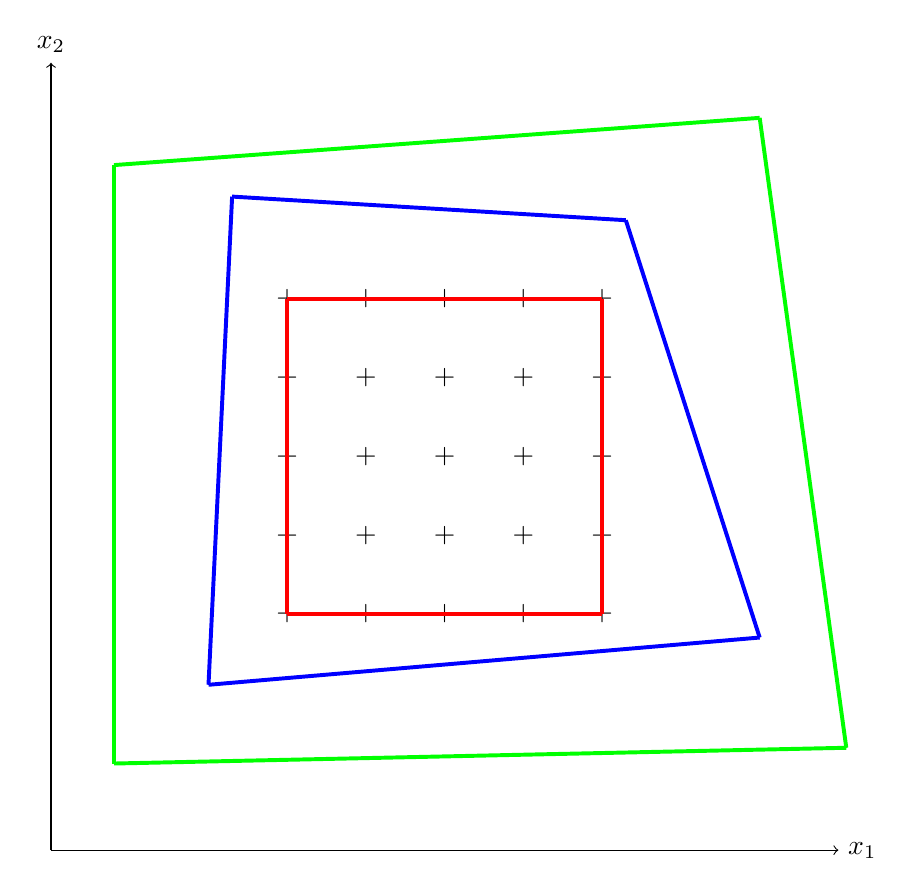
\begin{tikzpicture}
    
    \node (s1) at (3,3) {+};
    \node (s2) at (4,3) {+};
    \node (s3) at (5,3) {+};
    \node (s3) at (6,3) {+};    
    \node (s3) at (7,3) {+};
    \node (s1) at (3,4) {+};
    \node (s2) at (4,4) {+};
    \node (s3) at (5,4) {+};
    \node (s3) at (6,4) {+};    
    \node (s3) at (7,4) {+};   
    \node (s1) at (3,5) {+};
    \node (s2) at (4,5) {+};
    \node (s3) at (5,5) {+};
    \node (s3) at (6,5) {+};    
    \node (s3) at (7,5) {+};   
    \node (s1) at (3,6) {+};
    \node (s2) at (4,6) {+};
    \node (s3) at (5,6) {+};
    \node (s3) at (6,6) {+};    
    \node (s3) at (7,6) {+};   
    \node (s1) at (3,7) {+};
    \node (s2) at (4,7) {+};
    \node (s3) at (5,7) {+};
    \node (s3) at (6,7) {+};    
    \node (s3) at (7,7) {+};   

    \draw[-][line width=0.5mm, red ]  (3,3)--(7,3);
    \draw[-][line width=0.5mm, red ]  (7,7)--(7,3);
    \draw[-][line width=0.5mm, red ]  (3,3)--(3,7);
    \draw[-][line width=0.5mm, red ]  (3,7)--(7,7);

    \draw[-][line width=0.5mm, blue ]  (2,2.1)--(9,2.7);
    \draw[-][line width=0.5mm, blue ]  (2.3,8.3)--(7.3,8);
    \draw[-][line width=0.5mm, blue ]  (2,2.1)--(2.3,8.3);
    \draw[-][line width=0.5mm, blue ]  (7.3,8)--(9,2.7);
    
    \draw[-][line width=0.5mm, green ]  (0.8,1.1)--(10.1,1.3);
    \draw[-][line width=0.5mm, green ] (10.1,1.3)--(9,9.3);
    \draw[-][line width=0.5mm, green ]  (9,9.3)--(0.8, 8.7);
    \draw[-][line width=0.5mm, green ]  (0.8, 8.7)--(0.8,1.1);

    \draw[->] (0,0)--(0,10) node[above] {$x_2$};
    \draw[->] (0,0)--(10,0) node[right] {$x_1$};

    
    \end{tikzpicture} 
    

    \caption{Poliedros.}
    \label{poliedros}
\end{figure}

\section{Cortes no TSP}
Uma solução fracionária para a relaxação linear do TSP sem restrição de \textit{subtours} pode ser interpretada como um grafo completo. No grafo, todas as arestas terão um peso que varia de \(0\) a \(1\), e que obedecem às restrições de grau.
Suponha que, ao resolver a versão relaxada do TSP,  um \textit{solver} chegue a uma solução fracionária cujo corte mínimo é ilustrado na Figura \ref{fig:solucaoFrac}. Nela, o somatório dos pesos das arestas compartilhadas por \(S\) e \(\overline{S}\) é maior que \(2\). Isso significa que a solução, mesmo que fracionária, obedece a todas as restrições de \textit{subtour}, já que o corte mostrado é o menor possível. 

\begin{figure}[h]
    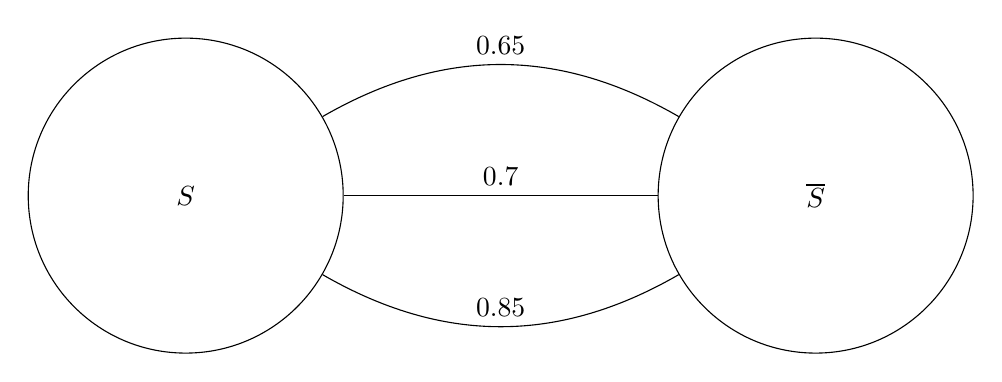
\begin{tikzpicture}
    
    \node[circle, draw=black, minimum size = 4cm] (s) at (0,0) {\(S\)};
    \node[circle, draw=black, minimum size = 4cm] (sbar) at (8,0) {\(\overline{S}\)};
    
    \path (s) edge node [above] {0.7}  (sbar); 
    \path [bend left] (s) edge node [above] {0.65} (sbar); 
    \path [bend right] (s) edge node [above] {0.85} (sbar);
    
    \end{tikzpicture}
    \caption{Solução fracionária para o TSP.}
    \label{fig:solucaoFrac}
\end{figure}

Se, no entanto, o somatório dos pesos das arestas fosse menor que 2, tanto \(S\) quanto \(\overline{S}\) estariam violando as restrições de \textit{subtour}, o que pode ser contornado adicionando-se a restrição \(\sum_{i \in S}\sum_{j \in \overline{S}}x_{ij} \geq 2\). Dessa forma, múltiplas restrições de \textit{subtour} podem ser adicionadas ao modelo antes mesmo de uma solução inteira ser obtida, além de aproximar o poliedro cada vez mais de sua envoltória convexa.

Conhecer o \textit{min-cut} do grafo que representa as soluções fracionárias da relaxação linear do TSP torna-se, portanto, uma vantagem.

\section{Algoritmos para a obtenção do \textit{min-cut}}

%O algoritmo proposto por \cite{Stoer:1997:SMA:263867.263872} é simples, e é capaz de encontrar o corte mínimo de um grafo de forma exata. A heurística \textit{max-back} descrita em \cite{denisnaddef}, por sua vez, é mais rápida que o algoritmo exato, embora não garanta a obtenção do \textit{min-cut}. Apesar disso, para soluções inteiras, é garantido que o \textit{max-back} resolve o problema da separação.

%Recomenda-se, primeiramente, o uso do \textit{max-back} na tentativa de detectar violações das restrições de \textit{subtour}. Se elas não forem encontradas, utiliza-se o algoritmo exato.

Nesta seção, serão descritos dois métodos para a obtenção do \textit{min-cut}. Precisamente, na Seção \ref{sec:maxBack}, será apresentada a heurística \textit{max-back} \cite{denisnaddef}, um método bastante eficiente para a obtenção de cortes que, embora não garanta a obtenção do corte mínimo, resolve o problema da separação para soluções inteiras. Por outro lado, na Seção \ref{sec:minCut}, é apresentado o algoritmo exato para obtenção do corte mínimo \cite{Stoer:1997:SMA:263867.263872}. Recomenda-se, primeiramente, o uso do \textit{max-back} na tentativa de detectar violações das restrições de \textit{subtour}. Se elas não forem encontradas, utiliza-se o algoritmo exato. Detalhes sobre a implementação serão discutidos na Seção \ref{sec:implementacao}.    

\subsection{Heurística \textit{Max-back}} \label{sec:maxBack}

\begin{algorithm}[h]
\DontPrintSemicolon
\KwData{..}
\KwResult{}
\Begin{

	\Return{} \;
}
\caption{\textsc{Max-back Heuristic}\label{alg:maxback}}
\end{algorithm}


\subsection{Algoritmo exato para o \textit{Min-cut}} \label{sec:minCut}

\begin{algorithm}[h]
\DontPrintSemicolon
\KwData{..}
\KwResult{}
\Begin{

	\Return{} \;
}
\caption{\textsc{Minimum Cut}\label{alg:maxback}}
\end{algorithm}

\subsection{Implementação} \label{sec:implementacao}

Neste seção, estão ressaltados os principais trechos de código que compõem a implementação do algoritmo \textit{Branch-and-Cut} aplicado ao TSP. O Código \ref{cod:modeloTSP}, por exemplo, apresenta o modelo para o TSP sem as restrições de proibição de \textit{subtours}. Note que são definidas as variáveis associadas às arestas presentes no grafo, a função objetivo como a minimização da distância total percorrida e apenas as restrições de grau.  

\begin{lstlisting}[style=cplusplusListStyle, caption= Modelo TSP sem as restrições de proibição de subtours, label=cod:modeloTSP]
    IloEnv env;
    IloModel model(env);

    env.setName("Branch and Cut");
    model.setName("Symmetrical Traveling Salesman Problem");

    int dimension = data->getDimension();

    /******** Creating one variable 'x' for each edge *******/
    IloArray <IloBoolVarArray> x(env, dimension);

    for (int i = 0; i < dimension; i++) {
        IloBoolVarArray array(env, dimension);
        x[i] = array;
    }

    /********** Adding variables 'x' to the model **********/
    char var[100];
    for (int i = 0; i < dimension; i++){
        for (int j = i + 1; j < dimension; j++){
            sprintf(var, "X(%d,%d)", i, j);
            x[i][j].setName(var);
            model.add(x[i][j]);
        }
    }
    
    /**************** Objective Function ******************/
    IloExpr obj(env);
    for (int i = 0; i < dimension; i++) {
        for (int j = i + 1; j < dimension; j++) {
            obj += data->getDistance(i, j)*x[i][j];
        }
    }
    model.add(IloMinimize(env, obj));
    
    /******************** Constraints *********************/
    IloRange r;
    char name[100];

    for (int i = 0; i < dimension; i++){
        IloExpr sumX(env);
        for (int j = 0; j < dimension; j++){
            if (j < i){
                sumX += x[j][i];
            }
            if (i < j){
                sumX += x[i][j];
            }
        }
        r = (sumX == 2);
        sprintf(name, "c_%d", i);
        r.setName(name);
        model.add(r);
    }
\end{lstlisting}

Definido o modelo, o próximo passo consiste na implementação dos cortes que proibirão soluções contendo \textit{subtours}. Para tanto, é preciso utilizar funções denominadas \textit{callbacks}. No escopo do resolvedor CPLEX, tais funções permitem que os usuários programem trechos de código que deverão ser executados durante a resolução do modelo \cite{CallbackCPLEX}. Precisamente, são utilizadas três classes de \textit{callbacks}, denominadas \emph{MyBranchCallback}, \emph{MyCutCallback} e \emph{MyLazyCallback}, cujos comandos para suas inicializações estão descritos no Código \ref{cod:comandosCallbacks}. 

\begin{lstlisting}[style=cplusplusListStyle, caption= Comandos do CPLEX para a utilização das \textit{callbacks}, label=cod:comandosCallbacks]
    // [...]
    
    IloCplex STSP(model);
    
    /********** Creating Branch Callback Object ***********/
    MyBranchCallback* branchCbk = new (env) MyBranchCallback(env);
    STSP.use(branchCbk);

    /************ Creating Cut Callback Object ************/
    MyCutCallback* cutCbk = new (env) MyCutCallback(env, x_ref, dimension);
    STSP.use(cutCbk);

    /************ Creating Lazy Callback Object ***********/
    MyLazyCallback* lazyCbk = new (env) MyLazyCallback(env, x_ref, dimension);
    STSP.use(lazyCbk);
    
    /**************** Cleaning the memory *****************/
    delete branchCbk;
    delete cutCbk;
    delete lazyCbk;
    env.end();

    // [...]
\end{lstlisting}

A classe \emph{MyBranchCallback} é utilizada para {\color{red}[...]}

\begin{lstlisting}[style=cplusplusListStyle, caption= Código referente à  classe \emph{MyBranchCallback}, label=cod:branchCallback]
MyBranchCallback::MyBranchCallback(IloEnv env) : IloCplex::BranchCallbackI(env) {}   

// returns a copy of the callback. Required by CPLEX
IloCplex::CallbackI* MyBranchCallback::duplicateCallback() const 
{ 
   return new (getEnv()) MyBranchCallback(getEnv()); 
}   

void MyBranchCallback::main()
{
	// How many branches would CPLEX create? 
	IloInt const nbranch = getNbranches(); 

	if(nbranch > 0){ 
		// CPLEX would branch. Get the branches CPLEX would create 
		// and create exactly those branches. With each branch store 
		// its NodeInfo. 
		// Note that getNodeData() returns NULL for the root node. 
		NodeInfo *data = dynamic_cast<NodeInfo *>(getNodeData()); 
		unsigned int depth;
   
		if(!data){
		   	// se entrou aqui e porque o no atual e a raiz. Cplex nao guarda NodeInfo para a raiz, por isso o metodo acima retorna NULL.
			// O NodeInfo da raiz e um objeto estatico da classe NodeInfo. Abaixo, verifica-se se objeto ja foi construido e aponta-se o ponteiro data para ele.
			if(NodeInfo::rootData == NULL){
				NodeInfo::initRootData();
			}
			data = NodeInfo::rootData;
		}

		depth = data->getDepth();

		IloNumVarArray vars(getEnv());
		IloNumArray bounds(getEnv()); 
		IloCplex::BranchDirectionArray dirs(getEnv());   

		//cria as mesmas branches que o cplex criaria, mas coloca o NodeInfo.
		for(IloInt i = 0; i < nbranch; ++i){ 
			IloNum const est = getBranch(vars, bounds, dirs, i);
			makeBranch(vars, bounds, dirs, est, new NodeInfo(depth + 1U)); 
		} 

		dirs.end(); 
		bounds.end(); 
		vars.end(); 
   } 
   else{ 
		// CPLEX would not create any branch here. Prune the node. 
		prune(); 
   } 
}

\end{lstlisting}

Por sua vez, a classe \emph{MyCutCallback} tem por finalidade {\color{red}[...]}

\begin{lstlisting}[style=cplusplusListStyle, caption= Código referente à  classe \emph{MyCutCallback}, label=cod:cutCallback]

/************************ Class' Constructor ************************/
MyCutCallback::MyCutCallback(IloEnv env, const IloArray<IloBoolVarArray>& x_ref, int nodes) : IloCplex::UserCutCallbackI(env), x(x_ref), x_vars(env), n(nodes)
{
	/********** Filling x_vars **********/ 
	for(int i = 0; i < n; i++) {
		for(int j = i + 1; j < n; j++){
			x_vars.add(x[i][j]);
		}
	}
	/************************************/
} 

/****** Return a callback copy. This method is a CPLEX requirement ******/
IloCplex::CallbackI* MyCutCallback::duplicateCallback() const 
{ 
   return new (getEnv()) MyCutCallback(getEnv(), x, n); 
}

/**************** Callback's code that is runned by CPLEX ***************/
void MyCutCallback::main() 
{
	/**************** Getting the node's depth ****************/
	//int depth = 0;
	/*NodeInfo *data = dynamic_cast<NodeInfo*>(getNodeData());

	if (!data){
        if (NodeInfo::rootData == NULL)
            NodeInfo::initRootData();
        
		data = NodeInfo::rootData;
    }
	if (data) {
		depth = data->getDepth();
	}*/
	int depth = getCurrentNodeDepth();
	/**********************************************************/

	/********** Getting the relaxed variables values **********/
	IloNumArray x_vals(getEnv(), (0.5*(n)*(n-1)));
	getValues(x_vals, x_vars);
	/**********************************************************/

	vector< vector<int> > cutSetPool;
	vector<IloConstraint> cons; 

	double **x_edge = new double*[n];
 
	for (int i = 0; i < n; i++) {
		x_edge[i] = new double[n];
	}

	int l = 0;
	for(int i = 0; i < n; i++) {
		for(int j = i+1; j < n; j++) {
			x_edge[i][j] = x_vals[l++];
		}
	}
	
	cutSetPool = MaxBack(x_edge, n);
	
	if (cutSetPool.empty() && depth <= 7) {
		cutSetPool = MinCut(x_edge, n);
		//cutSetPool = MultipleMinCut(x_edge, n);
	}

	/***************** Creating the constraints ***************/
	if (!cutSetPool.empty()){
		for (int c = 0; c < cutSetPool.size(); c++) {
			IloExpr p(getEnv());
			for(int i = 0; i < cutSetPool[c].size(); i++){
				for(int j = 0; j < cutSetPool[c].size(); j++){
					if(cutSetPool[c][i] < cutSetPool[c][j]){
						p += x[cutSetPool[c][i]][cutSetPool[c][j]];
					}
				}
			}
			int RHS = cutSetPool[c].size();
			cons.push_back(p <= RHS - 1);
		}
		/*********** Adding the constraints to the model **********/
		for(int i = 0; i < cons.size(); i++){
			add(cons.at(i)).end();
		}
		/**********************************************************/
	}
	/**********************************************************/

	/******************* Cleaning the memory ******************/
	for (int i = 0; i < n; i++) {
		delete[] x_edge[i];
	}
	delete[] x_edge;
	/**********************************************************/
}

\end{lstlisting}

Por fim, a classe \emph{MyLazyCallback} é necessária para {\color{red}[...]}

\begin{lstlisting}[style=cplusplusListStyle, caption= Código referente à  classe \emph{MyLazyCallback}, label=cod:lazyCallback]

\end{lstlisting}

{\color{red}Encerrar com um parágrafo de conclusão e indicando onde encontrar o código referente a estrutura completa (que está sendo compartilhado como arquivo zip por e-maail atualmente).}

% Códigos importantes

% 1 - Modelo sem as restrições de subtour: arquivo main.cpp
% 2 - Comandos do cplex para utilizar as callbacks: arquivo main.cpp
% 3 - Função main da classe MyLazyCallback: arquivo MyLazyCallback.cpp
% 4 - Função main da classe MyCutCallback: arquivo MyCutCallback.cpp
% 5 - Função main da classe MyBranchCallback: arquivo MyBranchCallback.cpp

% lstlistings: https://www.overleaf.com/learn/latex/Code_listing